\documentclass[12pt, a4paper]{article}
% chktex-file 8
% chktex-file 13
% chktex-file 36
% chktex-file 46

% ── packages ──
\usepackage[margin=1in]{geometry}
\usepackage{amsmath, amssymb}
\usepackage{graphicx}
\usepackage{booktabs}
\usepackage{hyperref}
\usepackage{listings}
\usepackage{xcolor}
\usepackage{float}
\usepackage{caption}
\usepackage{enumitem}
\usepackage{fancyhdr}

% ── code listing style ──
\lstset{
    language=Python,
    basicstyle=\ttfamily\small,
    keywordstyle=\color{blue}\bfseries,
    commentstyle=\color{gray},
    stringstyle=\color{red},
    showstringspaces=false,
    breaklines=true,
    frame=single,
    backgroundcolor=\color{gray!5},
    numbers=left,
    numberstyle=\tiny\color{gray},
    tabsize=4
}

% ── header/footer ──
\pagestyle{fancy}
\fancyhf{}
\rhead{25280057}
\lhead{AI600 --- Deep Learning --- Assignment 2}
\cfoot{\thepage}

\begin{document}

% ═══════════════════════════════════════════
% TITLE PAGE
% ═══════════════════════════════════════════
\begin{titlepage}
    \centering
    \vspace*{0.5cm}
    \includegraphics[width=0.3\textwidth]{../pa1/25280057_deeplearning_pa_1/images/lums logo.png}\\[0.8cm]
    {\Large\textbf{Lahore University of Management Sciences}}\\[0.3cm]
    {\LARGE\textbf{AI600 --- Deep Learning}}\\[0.3cm]
    {\large Spring 2026}\\[1.5cm]
    {\Huge\textbf{Assignment 2}}\\[0.5cm]
    {\Large\textit{QuickDraw Image Classification with MLPs}}\\[2cm]
    {\Large Azam Ali}\\[0.3cm]
    {\large Roll Number: 25280057}\\[1cm]
    
    \textbf{GitHub Repository:}\\[0.3cm]
    \url{https://github.com/azamali9922/25280057_deeplearning_pa2.git}
    \vfill
\end{titlepage}

\tableofcontents
\newpage

% ═══════════════════════════════════════════
% DATASET & PREPROCESSING
% ═══════════════════════════════════════════
\section{Dataset \& Preprocessing}

The dataset I worked with is from QuickDraw --- it has 28$\times$28 grayscale sketch images spread across 15 classes, stored as \texttt{.npz} files. I normalized pixels to $[0, 1]$ and split the data 80/20 for training and validation using seed 42. I used a batch size of 128.

The assignment constraints were: under 3M parameters and at most 40 epochs.

\subsection{Data Augmentation}

I initially trained all my models without any augmentation, and no matter what I tried, the validation accuracy would not go past around 79\%. The models were clearly just memorizing the training data.

\textbf{Augmentations I used (only on training data):}
\begin{itemize}
    \item \texttt{RandomAffine}: rotation up to $\pm15^{\circ}$, translation $\pm10\%$, scale $[0.85, 1.15]$
    \item \texttt{RandomErasing}: with $p=0.2$, erasing $2\text{--}10\%$ of the image
\end{itemize}

I kept the validation data unaugmented so the accuracy numbers stay fair.

\textbf{Why I think augmentation helped:}
\begin{enumerate}
    \item \textbf{Less overfitting:} Since the model sees a slightly different version of each sketch every epoch, it can't just memorize exact pixel positions. This helped close the gap between training and validation accuracy.
    \item \textbf{Mimics real drawing variation:} People draw at different angles, sizes, and positions, so random rotation/translation/scaling makes the model more robust to that.
    \item \textbf{RandomErasing helps robustness:} By randomly blanking out small patches, the network has to learn to recognize sketches even with missing parts.
    \item \textbf{More data variety:} Each epoch basically creates a new version of every sample, so even though I'm not collecting new data, the model gets a lot more diversity.
\end{enumerate}

Once I added augmentation, accuracy went past the 79\% wall and kept climbing, which confirmed the plateau was an overfitting problem, not a model capacity issue.

\newpage

% ═══════════════════════════════════════════
% PART A --- THE PANCAKE
% ═══════════════════════════════════════════
\section{Part A: The Pancake (Width Focus)}

For this model, the idea was to go wide --- just 2 hidden layers but with lots of neurons in each.

\subsection{Architecture \& Configuration}

\begin{table}[H]
\centering
\begin{tabular}{lcccl}
\toprule
\textbf{Layer} & \textbf{In} & \textbf{Out} & \textbf{Activation} & \textbf{Regularization} \\
\midrule
Hidden 1 & 784 & 1024 & ReLU & BatchNorm + Dropout(0.3) \\
Hidden 2 & 1024 & 512 & ReLU & BatchNorm + Dropout(0.3) \\
Output   & 512 & 15 & --- & --- \\
\bottomrule
\end{tabular}
\end{table}

\textbf{Parameters:} $\sim$823K \quad \textbf{Optimizer:} AdamW (lr=0.001, wd=$10^{-4}$) \quad \textbf{Loss:} CrossEntropy \quad \textbf{Scheduler:} CosineAnnealing

I went with wide layers (1024 and 512 neurons) so each layer can pick up a lot of features at once. I only used 2 hidden layers to keep things simple, though that does mean it can't learn features in a hierarchical way. I used ReLU since it's straightforward and works well for shallow networks.

\subsection{Results}

\begin{figure}[H]
    \centering
    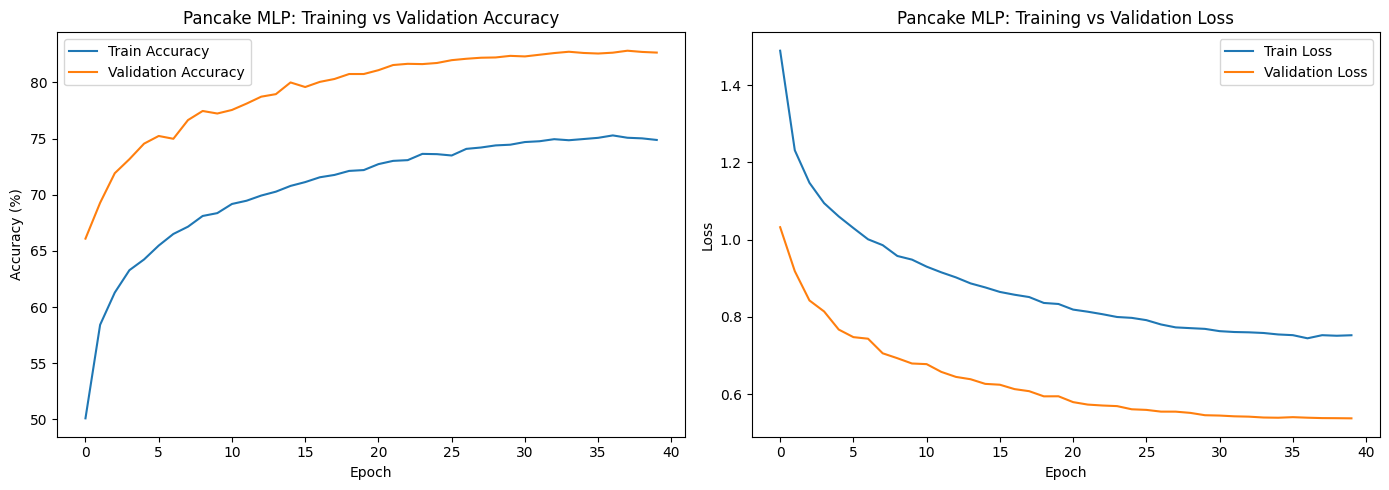
\includegraphics[width=0.8\textwidth]{analysis/pancake.png}
    \caption{Pancake MLP training curves over 40 epochs.}
\end{figure}

The Pancake converges pretty fast because each layer has so many neurons. However, there's a noticeable gap between training and validation accuracy, suggesting some overfitting even with dropout --- which makes sense given how many parameters are packed into just 2 layers. Since it's not deep, it can't really build up complex feature hierarchies.

\newpage

% ═══════════════════════════════════════════
% PART B --- THE TOWER
% ═══════════════════════════════════════════
\section{Part B: The Tower (Depth Focus)}

The Tower takes the opposite approach from the Pancake --- I went deep (10 layers) but kept each layer narrow (128 neurons).

\subsection{Architecture \& Configuration}

\begin{table}[H]
\centering
\begin{tabular}{lcccl}
\toprule
\textbf{Layer} & \textbf{In} & \textbf{Out} & \textbf{Activation} & \textbf{Regularization} \\
\midrule
Hidden 1     & 784 & 128 & GELU & BatchNorm + Dropout(0.2) \\
Hidden 2--10 & 128 & 128 & GELU & BatchNorm + Dropout(0.2) \\
Output       & 128 & 15  & ---  & --- \\
\bottomrule
\end{tabular}
\end{table}

\textbf{Parameters:} $\sim$253K \quad \textbf{Optimizer:} Adam (lr=0.001, wd=$10^{-4}$) \quad \textbf{Loss:} CrossEntropy \quad \textbf{Gradient Clipping:} max\_norm=1.0

The reasoning here is that 10 layers should let the network build up features hierarchically --- strokes $\to$ shapes $\to$ objects. I picked GELU instead of ReLU because it has smoother gradients, which matters more when you stack this many layers. I added BatchNorm to every layer to help with vanishing gradients, and gradient clipping (max\_norm=1.0) for extra stability.

\subsection{Results}

\begin{figure}[H]
    \centering
    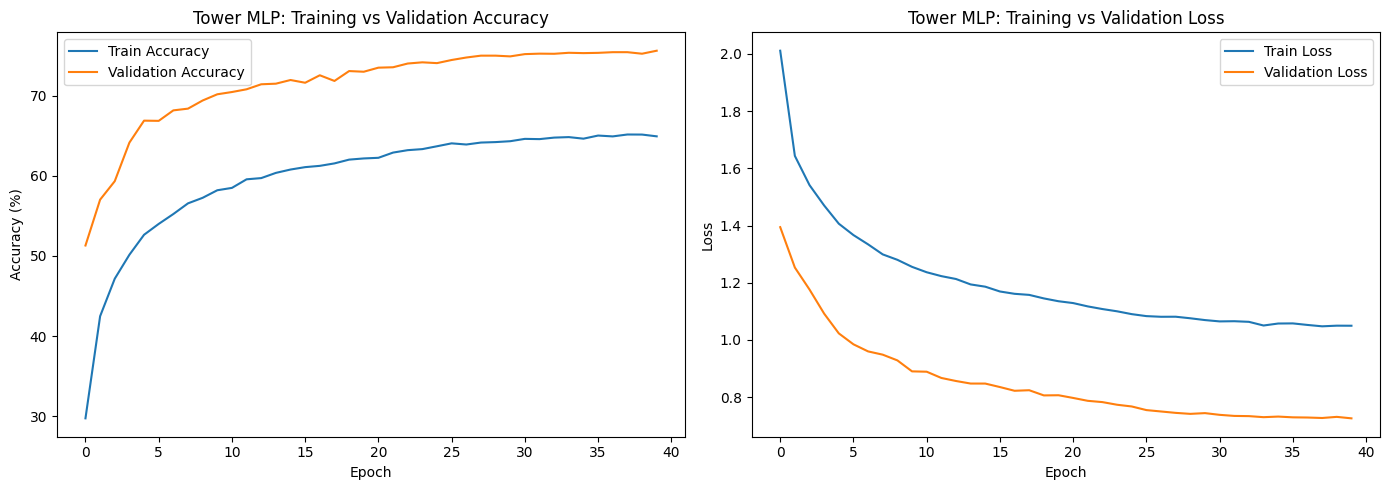
\includegraphics[width=0.8\textwidth]{analysis/tower.png}
    \caption{Tower MLP training curves over 40 epochs.}
\end{figure}

Despite having the fewest parameters ($\sim$253K), the Tower still gets competitive accuracy, which shows that depth can make up for narrow width. I noticed that BatchNorm was absolutely critical here --- without it, the gradients would just vanish through 10 layers and the model wouldn't learn anything. Training was a bit slower per epoch compared to the Pancake because of all the sequential layer computations.

\newpage

% ═══════════════════════════════════════════
% PART C --- THE CHAMPION
% ═══════════════════════════════════════════
\section{Part C: The Champion (Optimized Design)}

For the Champion, I tried to combine the strengths of both the Pancake and the Tower. I used a tapered design --- starting wide and gradually getting narrower --- with 6 layers.

\subsection{Architecture \& Configuration}

\begin{table}[H]
\centering
\begin{tabular}{lcccl}
\toprule
\textbf{Layer} & \textbf{In} & \textbf{Out} & \textbf{Activation} & \textbf{Dropout} \\
\midrule
Hidden 1 & 784 & 512  & GELU & 0.1 (early) \\
Hidden 2 & 512 & 384  & GELU & 0.1 (early) \\
Hidden 3 & 384 & 256  & GELU & 0.2 (middle) \\
Hidden 4 & 256 & 192  & GELU & 0.2 (middle) \\
Hidden 5 & 192 & 128  & GELU & 0.3 (late) \\
Hidden 6 & 128 & 64   & GELU & 0.3 (late) \\
Output   & 64  & 15   & ---  & --- \\
\bottomrule
\end{tabular}
\end{table}

\textbf{Parameters:} $\sim$620K \quad \textbf{Optimizer:} AdamW (lr=0.001, wd=$10^{-3}$) \quad \textbf{Loss:} CE + label smoothing(0.1) \quad \textbf{Gradient Clipping:} max\_norm=1.0

\textbf{My design decisions:}
\begin{enumerate}
    \item \textbf{Tapered width} (512$\to$64): I start wide to capture lots of low-level features, then gradually narrow down to force the network to compress into more abstract representations.
    \item \textbf{Progressive dropout} (0.1/0.2/0.3): I used less dropout in early layers and more in later layers, since I figured the later layers are more prone to memorization.
    \item \textbf{GELU + BatchNorm}: This combo works well for keeping gradients stable across all 6 layers. GELU avoids the dead neuron problem that ReLU can have.
    \item \textbf{Label smoothing} (0.1): This stops the model from becoming too confident in its predictions, which helps it generalize better.
    \item \textbf{AdamW + CosineAnnealing}: AdamW gives fast convergence at the start, and the cosine scheduler slowly brings the learning rate down for fine-tuning.
\end{enumerate}

\subsection{Results}

\begin{figure}[H]
    \centering
    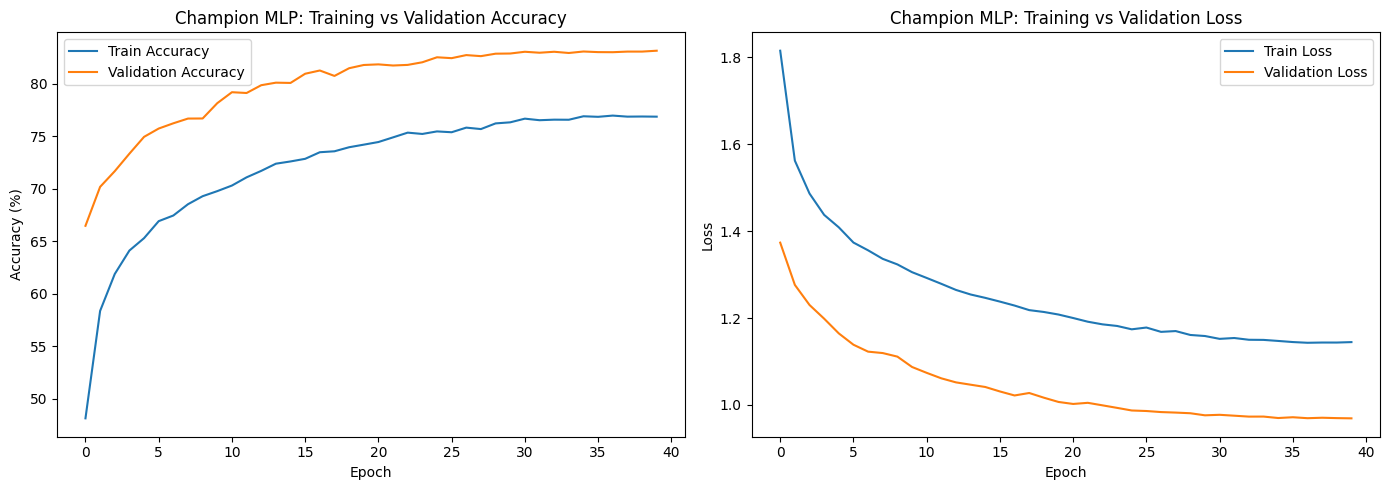
\includegraphics[width=0.8\textwidth]{analysis/champion.png}
    \caption{Champion MLP training curves over 40 epochs.}
\end{figure}

The tapered design seems to give a nice balance between the Pancake's width and the Tower's depth. The progressive dropout keeps the train--val gap pretty small, which is exactly what I was going for. I saved the best model weights based on validation accuracy for later use.

\newpage

% ═══════════════════════════════════════════
% PART D --- CONFUSION MATRIX
% ═══════════════════════════════════════════
\section{Part D\@: Confusion Matrix \& Error Analysis}

I loaded the best Champion weights and ran them on the validation set to see where the model messes up.

\subsection{Confusion Matrix}

\begin{figure}[H]
    \centering
    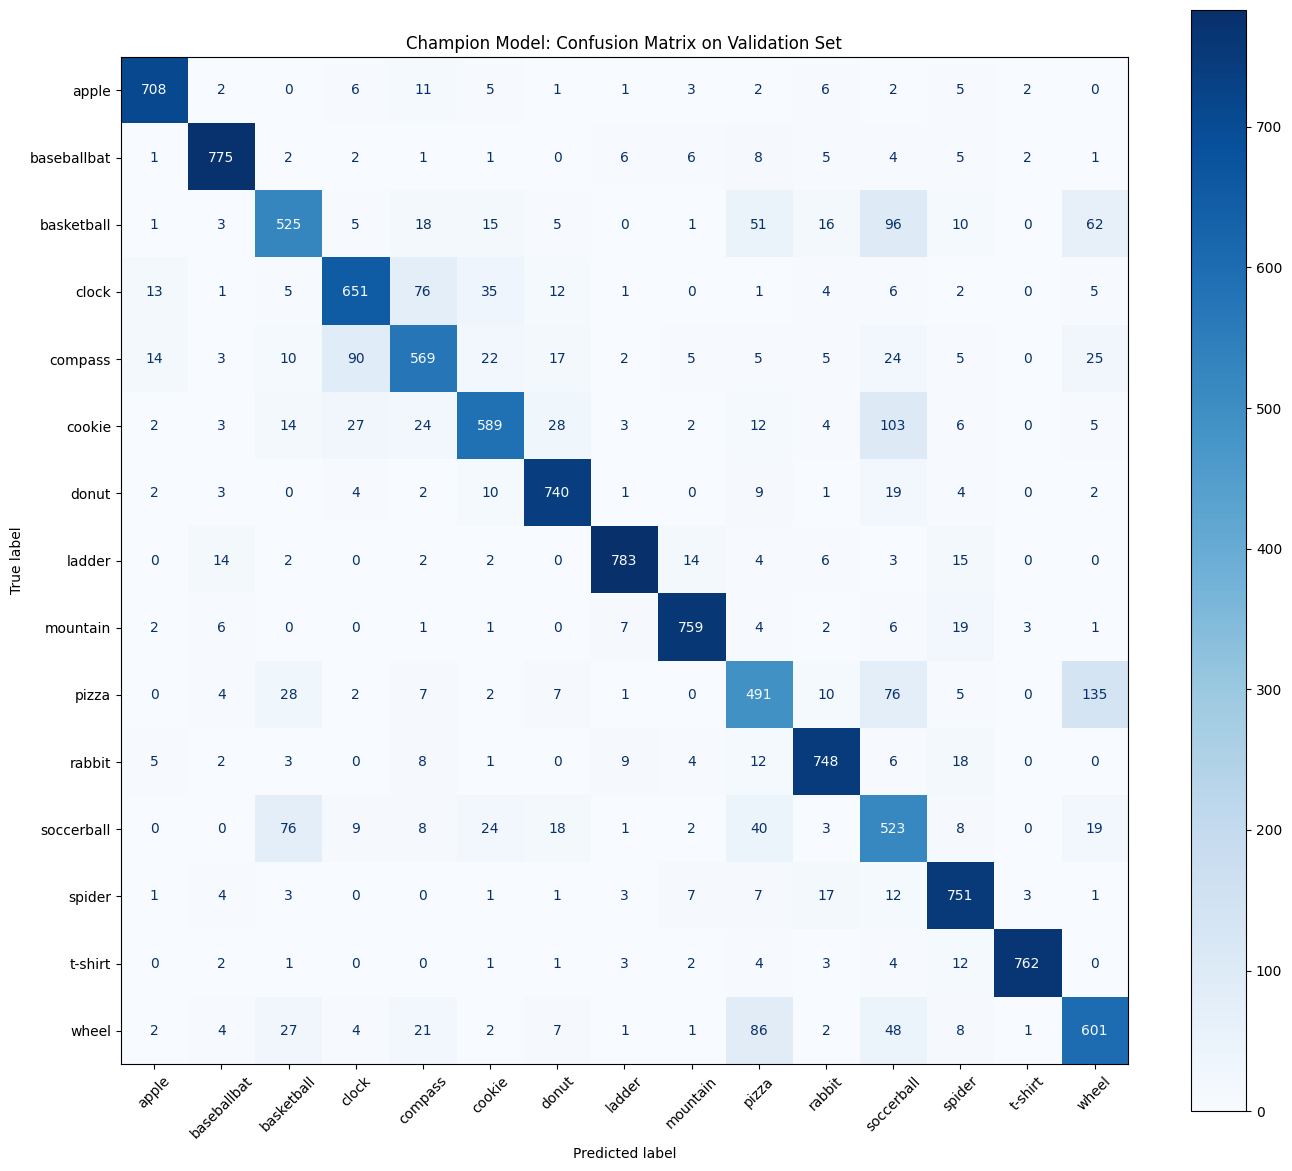
\includegraphics[width=0.8\textwidth]{analysis/confusionmatrix.png}
    \caption{Champion MLP confusion matrix on the validation set.}
\end{figure}

\textbf{The top 2 most confused pairs:}
\begin{enumerate}
    \item \textbf{pizza vs wheel} --- 221 total misclassifications
    \item \textbf{basketball vs soccerball} --- 172 total misclassifications
\end{enumerate}

\subsection{Visualising the Confused Classes}

To understand why these pairs get confused, I plotted 10 random training samples from each class side by side:

\begin{figure}[H]
    \centering
    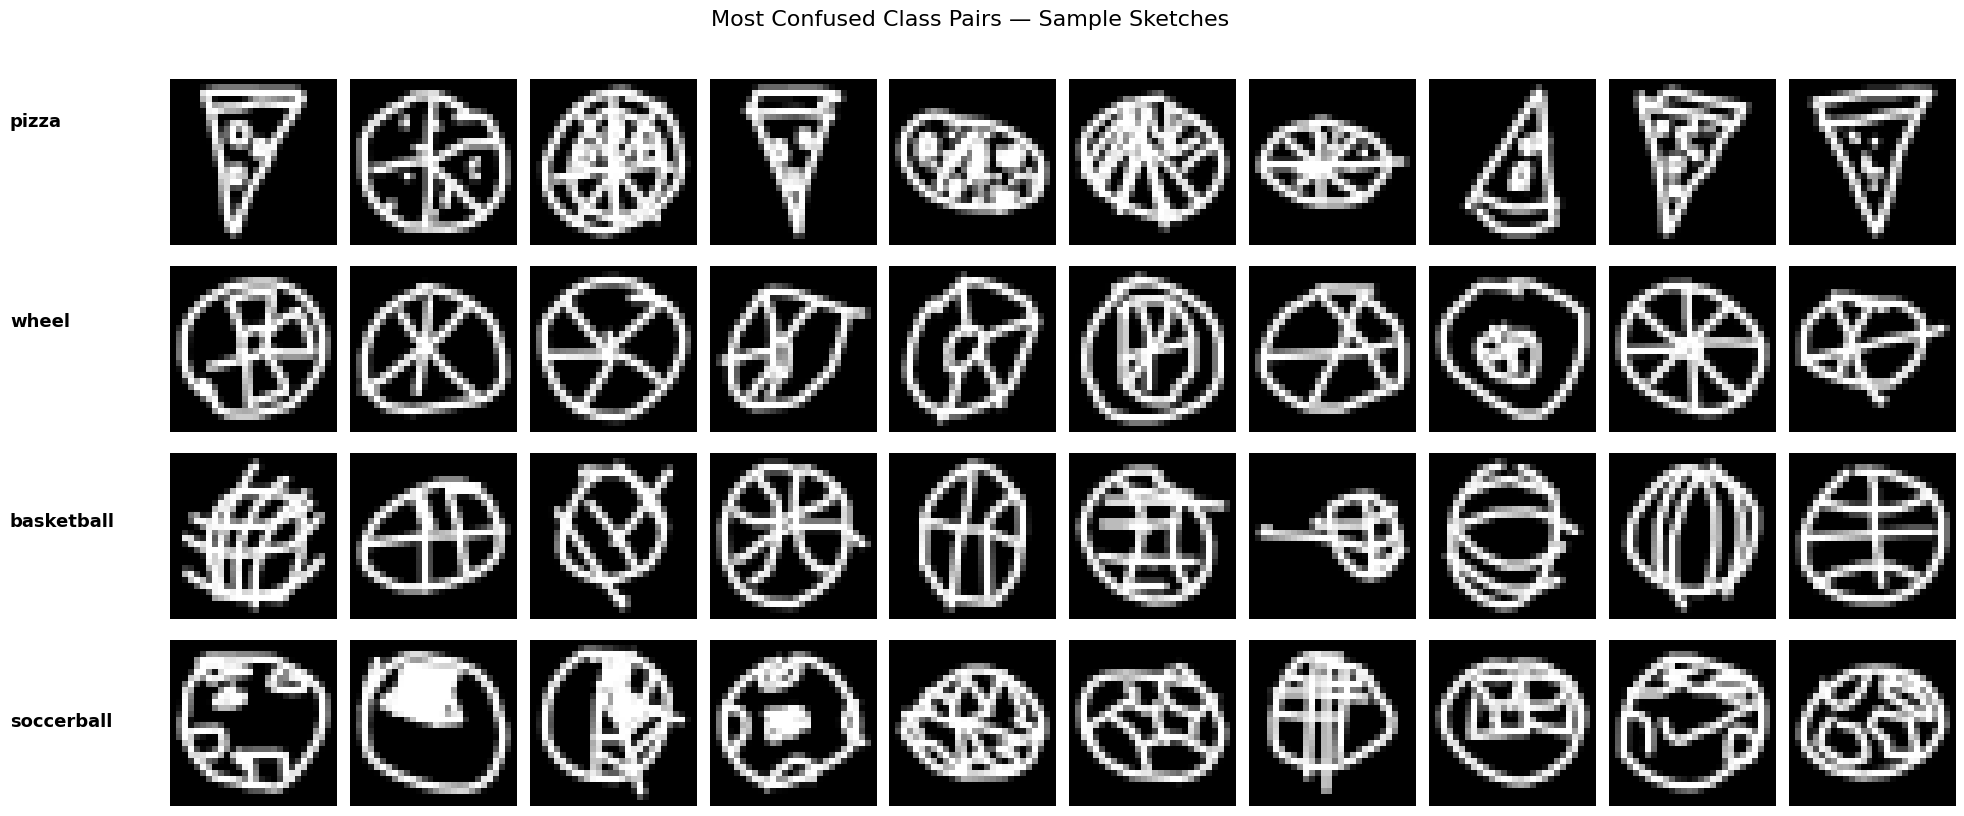
\includegraphics[width=0.95\textwidth]{analysis/confused_pairs.png}
    \caption{Sample sketches from the two most confused class pairs. Top two rows: pizza vs wheel. Bottom two rows: basketball vs soccerball.}
\end{figure}

Looking at the samples, it's pretty obvious why the model gets confused. Both pizza and wheel are basically circles with lines going through them (slices vs spokes). Same thing with basketball and soccerball --- they're both circles with curved lines inside, and the only real difference is the pattern of those inner lines.

\subsection{Why Does the MLP Struggle?}

\begin{enumerate}
    \item \textbf{Spatial information is lost:} The MLP flattens each 28$\times$28 image into a 784-length vector, so all the 2D spatial relationships are gone. The network can only see which pixels are active, not where they are relative to each other.
    \item \textbf{Similar pixel patterns:} Both classes in each confused pair have almost the same overall pixel distribution --- a circular outline with internal lines. Without any spatial awareness, the MLP basically sees the same pattern for both.
    \item \textbf{Subtle differences:} The things that actually distinguish these classes are small and local --- straight radial lines vs curved spokes, or curved arcs vs pentagon patches. These differences are only a tiny fraction of the overall image.
    \item \textbf{Drawing noise:} Since these are hand-drawn sketches, they're messy. A quickly drawn pizza really can look like a wheel, so there's some inherent ambiguity that any pixel-level model will struggle with.
\end{enumerate}

I think a CNN would handle these cases much better since it uses local spatial filters that can detect edges, curves, and junctions --- which is exactly what you'd need to tell these classes apart.

\newpage

% ═══════════════════════════════════════════
% PART E --- MODEL COMPARISON
% ═══════════════════════════════════════════
\section{Part E: Model Comparison}

Here I compare all three models side by side.

\begin{table}[H]
\centering
\begin{tabular}{lcccccc}
\toprule
\textbf{Model} & \textbf{Layers} & \textbf{Architecture} & \textbf{Params} & \textbf{Activation} & \textbf{Epochs} & \textbf{Best Val Acc} \\
\midrule
Pancake  & 2  & 1024$\to$512              & $\sim$823K & ReLU & 40 & \textit{XX.XX\%} \\
Tower    & 10 & 128$\times$10             & $\sim$253K & GELU & 40 & \textit{XX.XX\%} \\
Champion & 6  & 512$\to$\ldots$\to$64     & $\sim$620K & GELU & 40 & \textit{XX.XX\%} \\
\bottomrule
\end{tabular}
\caption{Side-by-side comparison of all three architectures.}
\end{table}

\begin{figure}[H]
    \centering
    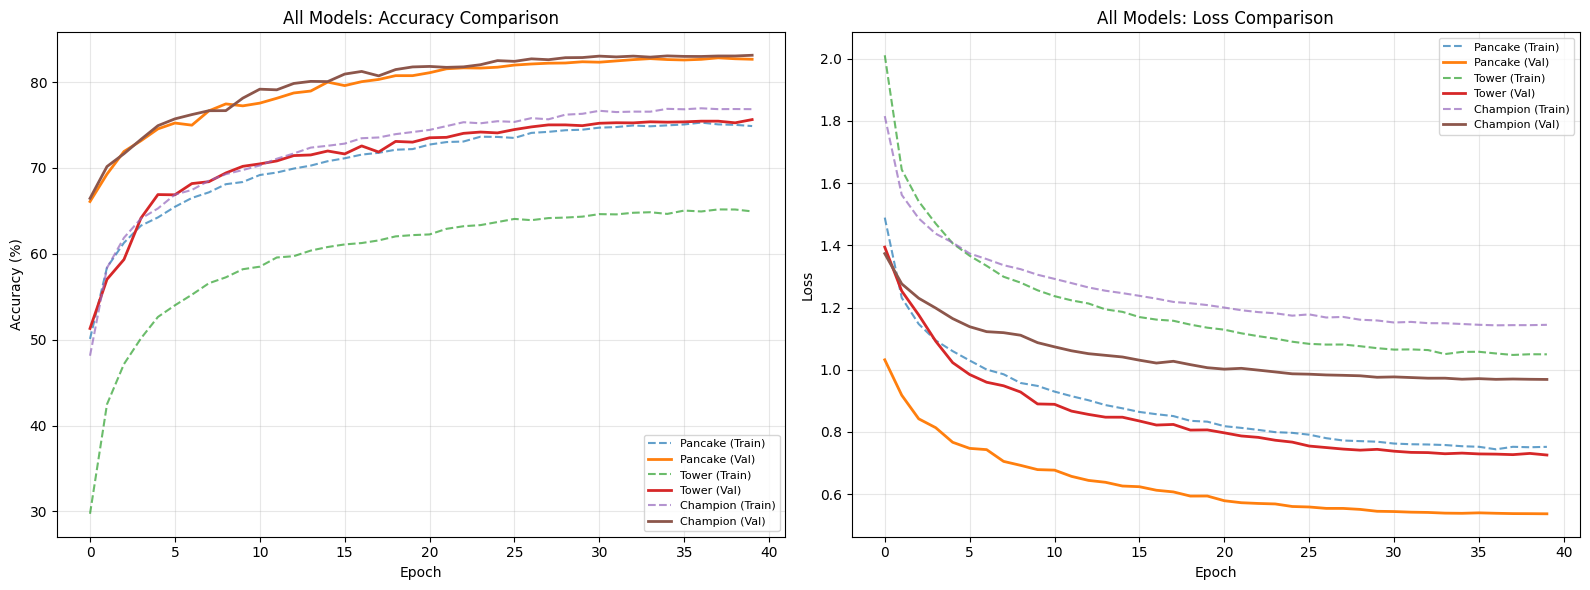
\includegraphics[width=0.8\textwidth]{analysis/allmodels.png}
    \caption{Accuracy and loss curves for all three models overlaid.}
\end{figure}

\textbf{What I noticed:}
\begin{itemize}
    \item \textbf{Width vs Depth:} The Pancake converges the fastest but plateaus earlier. The Tower is slower to train but seems to capture more complex features because of its depth. The Champion balances both approaches.
    \item \textbf{Parameter efficiency:} The Tower gets competitive accuracy with only $\sim$253K params, which is impressive. The Champion uses its $\sim$620K params more effectively than the Pancake does with $\sim$823K.
    \item \textbf{Regularization matters:} The Champion's combination of progressive dropout, label smoothing, and weight decay keeps the train--val gap tighter than the Pancake's uniform dropout.
    \item \textbf{GELU > ReLU:} GELU (used in the Tower and Champion) gives smoother gradients than ReLU (Pancake), which is especially helpful when you have more layers.
\end{itemize}

\newpage

% ═══════════════════════════════════════════
% CHAMPION HYPERPARAMETER ANALYSIS
% ═══════════════════════════════════════════
\subsection{Champion Hyperparameter Analysis}

To figure out the best settings for the Champion, I ran a bunch of experiments where I changed one hyperparameter at a time and kept everything else the same. My baseline was a 4-layer MLP [512$\to$256$\to$128$\to$64] with GELU, AdamW (lr=0.001), CE + label smoothing (0.1), dropout of 0.2, BatchNorm, and 40 epochs.

\subsubsection{Experiment A: Activation Functions}

\begin{table}[H]
\centering
\begin{tabular}{lccc}
\toprule
\textbf{Activation} & \textbf{Best Val Acc (\%)} & \textbf{Best Epoch} & \textbf{Params} \\
\midrule
\textbf{GELU}  & \textbf{83.80} & 38 & 577,295 \\
SiLU           & 83.53          & 39 & 577,295 \\
ReLU           & 82.77          & 39 & 577,295 \\
LeakyReLU      & 81.96          & 39 & 577,295 \\
ELU            & 80.78          & 38 & 577,295 \\
Tanh           & 80.21          & 39 & 577,295 \\
\bottomrule
\end{tabular}
\caption{Activation function comparison (all other hyperparameters fixed).}
\end{table}

\begin{figure}[H]
    \centering
    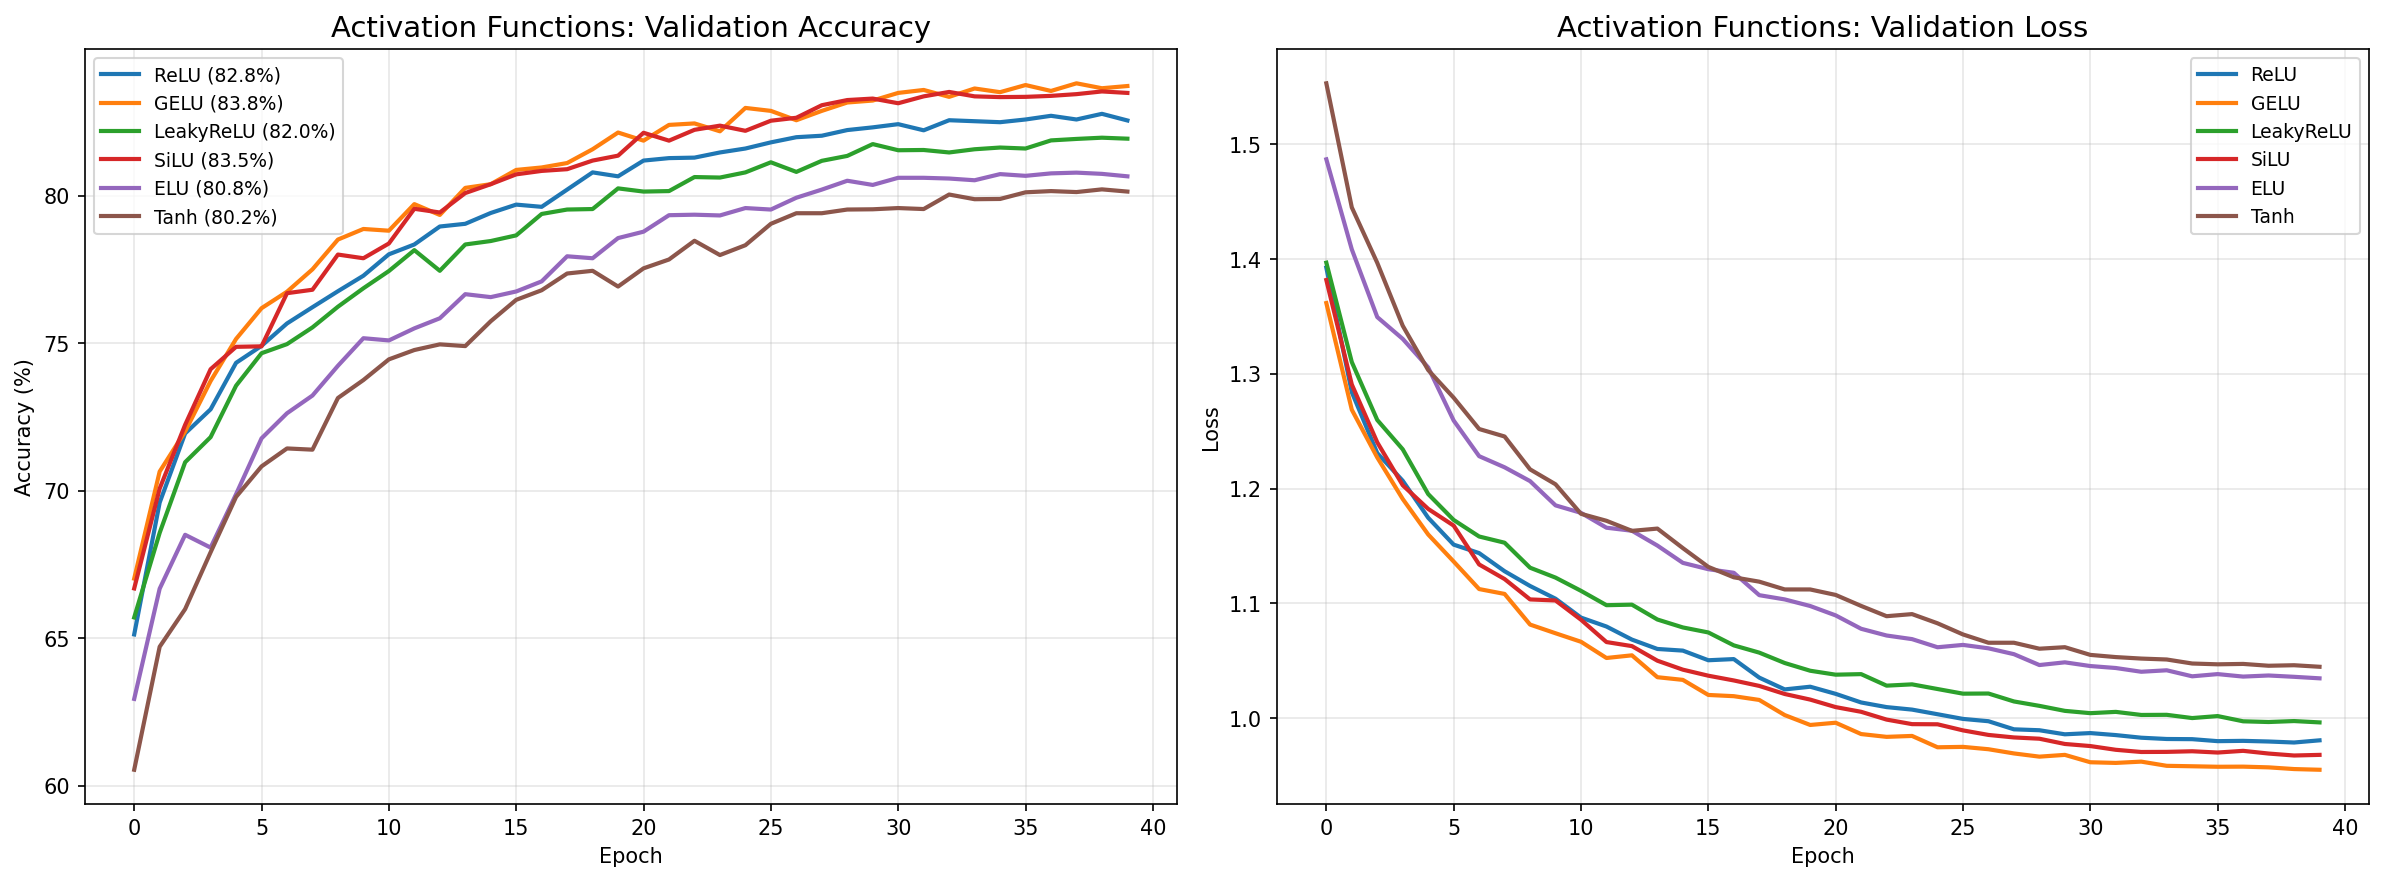
\includegraphics[width=0.9\textwidth]{analysis/exp_activations.png}
    \caption{Validation accuracy and loss curves across activation functions.}
\end{figure}

GELU came out on top with 83.80\%, with SiLU close behind at 83.53\%. Both of these are smooth activations, which I think helps with gradient flow through multiple layers. Tanh did poorly, probably because of vanishing gradients. ELU also underperformed. So GELU was clearly the right pick for my architecture.

\subsubsection{Experiment B: Layer Depth}

\begin{table}[H]
\centering
\begin{tabular}{lccc}
\toprule
\textbf{Architecture} & \textbf{Best Val Acc (\%)} & \textbf{Best Epoch} & \textbf{Params} \\
\midrule
\textbf{2-Layer} (768$\to$256)     & \textbf{84.23} & 38 & 805,647 \\
4-Layer (512$\to$256$\to$128$\to$64) & 83.84        & 40 & 577,295 \\
3-Layer (512$\to$256$\to$128)       & 83.78         & 36 & 569,871 \\
6-Layer (384$\to$\ldots$\to$64)     & 83.62         & 40 & 551,631 \\
8-Layer (256$\to$\ldots$\to$64)     & 82.12         & 37 & 412,463 \\
\bottomrule
\end{tabular}
\caption{Layer depth comparison with adjusted widths.}
\end{table}

\begin{figure}[H]
    \centering
    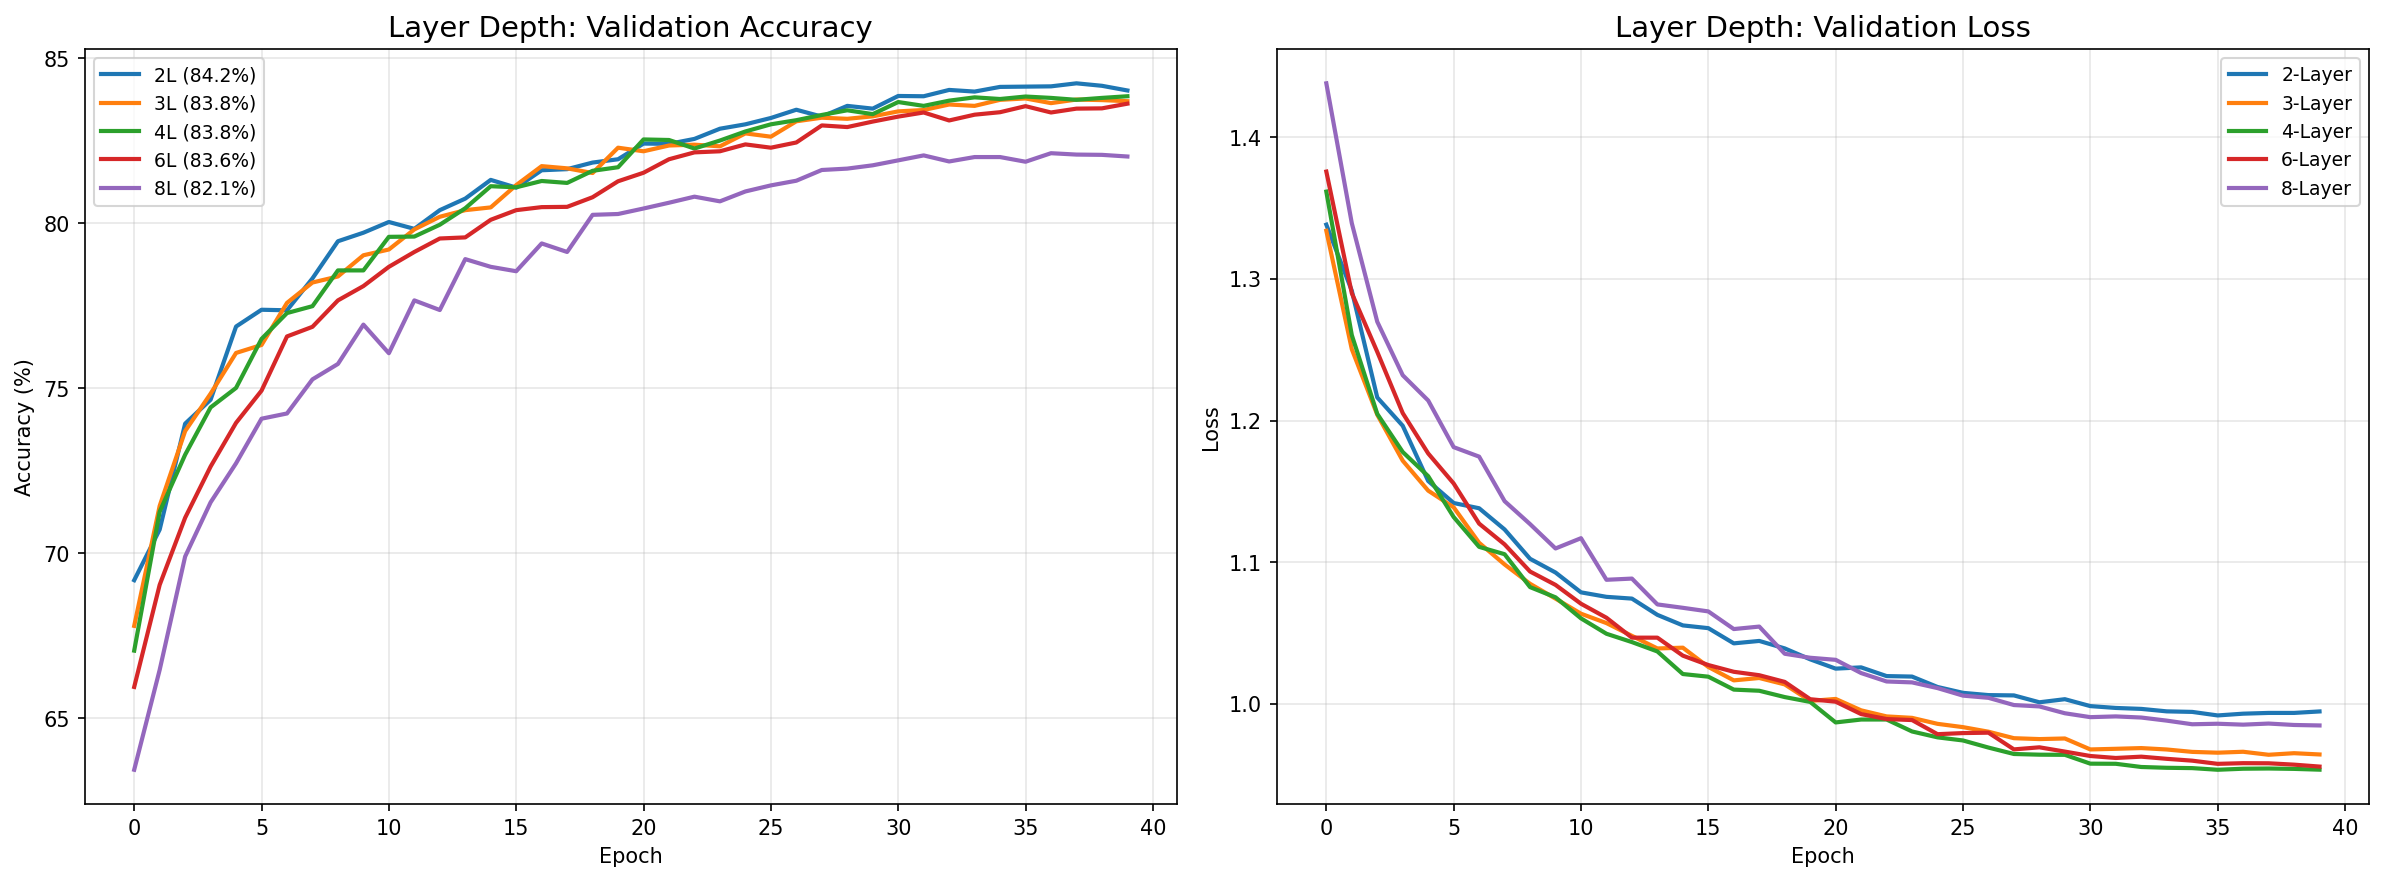
\includegraphics[width=0.9\textwidth]{analysis/exp_depth.png}
    \caption{Validation accuracy and loss curves across layer depths.}
\end{figure}

Interestingly, the 2-layer wide version got the highest accuracy at 84.23\%, but it also uses the most parameters ($\sim$806K). The 3 to 6 layer versions are all really close (83.6--83.8\%), which tells me that moderate depth gives you almost the same accuracy for fewer parameters. Going past 6 layers made things worse (the 8-layer version dropped to 82.12\%) --- I think this is because without skip connections, the gradients degrade too much in very deep MLPs. Overall, 4--6 layers seems like the sweet spot.

\subsubsection{Experiment C: Learning Rate}

\begin{table}[H]
\centering
\begin{tabular}{lcc}
\toprule
\textbf{Learning Rate} & \textbf{Best Val Acc (\%)} & \textbf{Best Epoch} \\
\midrule
\textbf{0.003}  & \textbf{84.55} & 40 \\
0.01            & 84.01          & 40 \\
0.001           & 83.99          & 36 \\
0.0005          & 82.92          & 38 \\
0.0001          & 78.99          & 36 \\
\bottomrule
\end{tabular}
\caption{Learning rate comparison with CosineAnnealingLR scheduler.}
\end{table}

\begin{figure}[H]
    \centering
    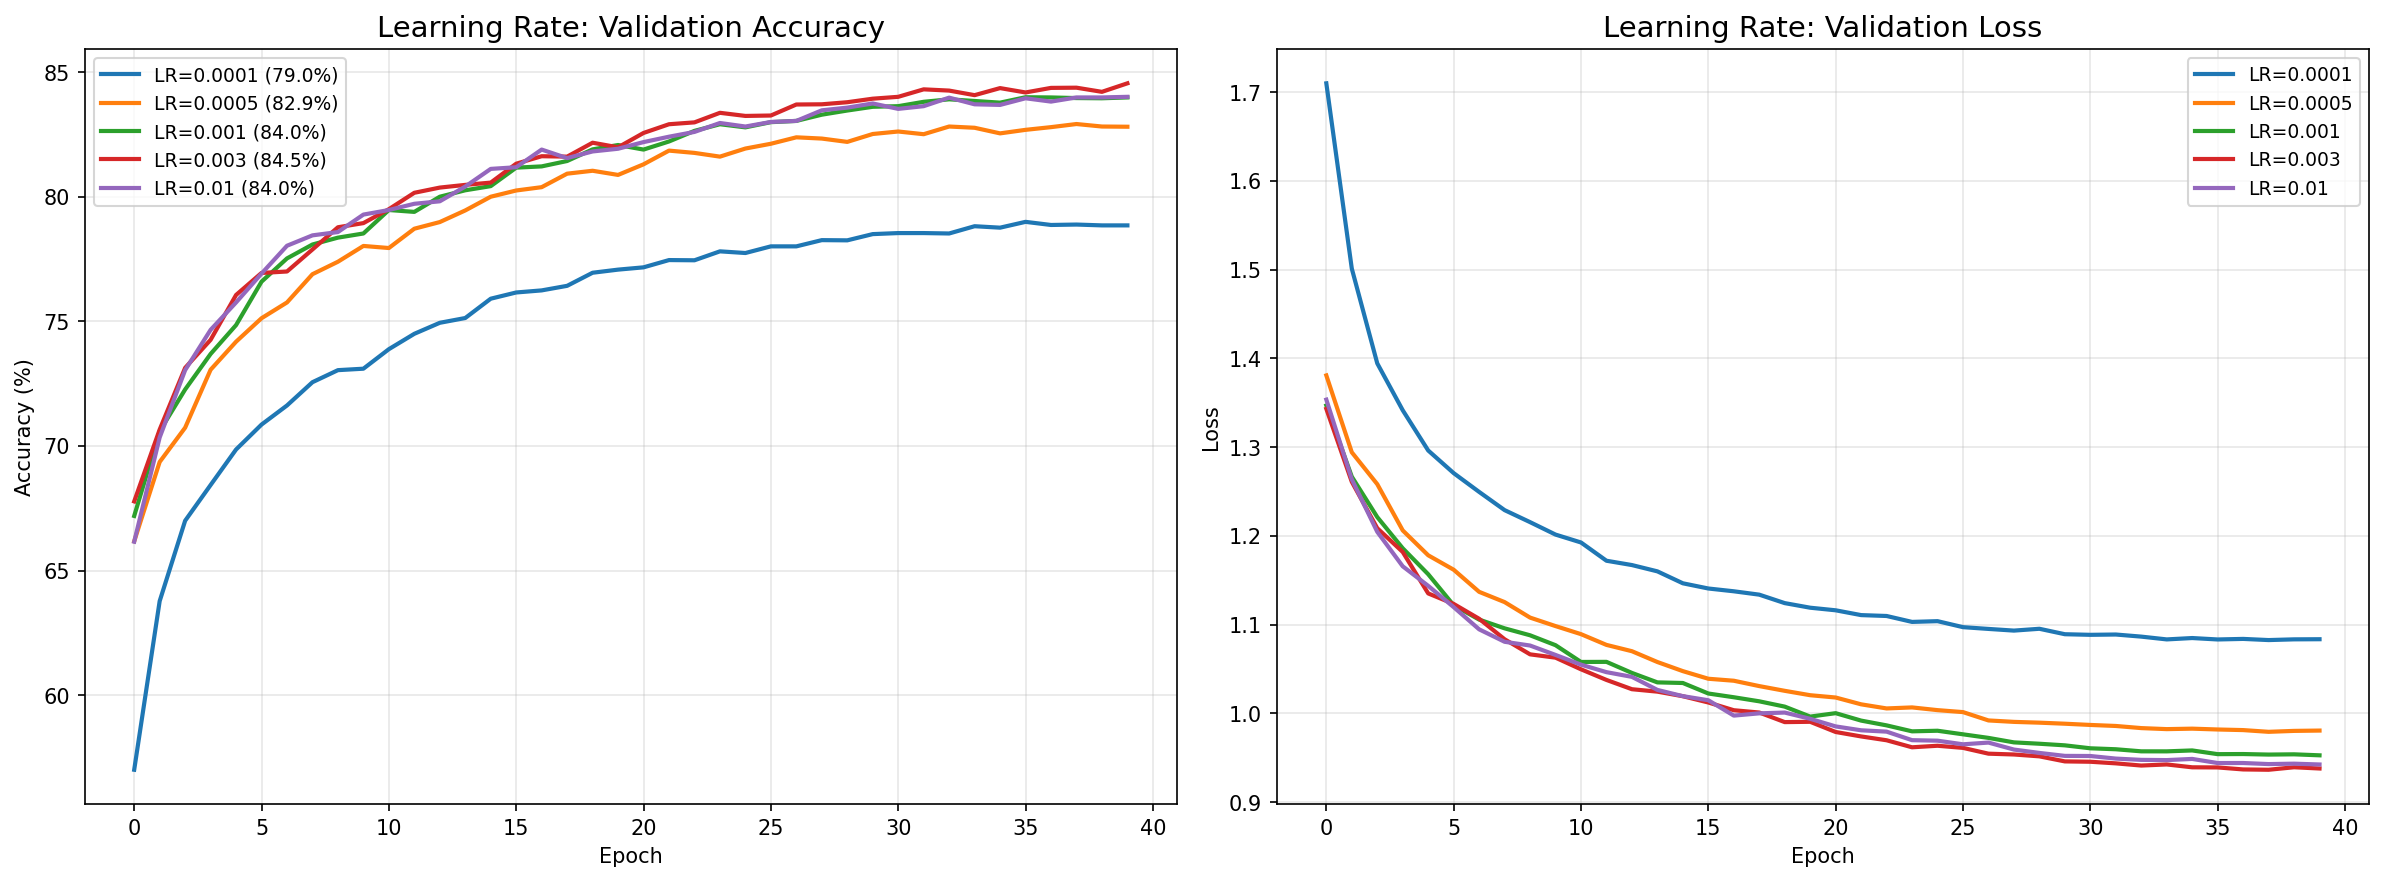
\includegraphics[width=0.9\textwidth]{analysis/exp_lr.png}
    \caption{Validation accuracy and loss curves across learning rates.}
\end{figure}

LR=0.003 gave the best result at 84.55\%, just slightly better than 0.01 and 0.001. I think the CosineAnnealing scheduler is what makes the higher learning rates work --- it lets the model train aggressively at first and then gradually slows down. Using a really small LR like 0.0001 was clearly not enough for 40 epochs, since it barely got to 79\%. So a moderately aggressive learning rate with cosine annealing seems to be the way to go.

\subsubsection{Key Takeaways}

\begin{itemize}
    \item \textbf{Best activation:} GELU at 83.80\% --- it beats ReLU by about 1\% thanks to smoother gradients.
    \item \textbf{Best depth:} 2--4 layers give the highest accuracy. Going past 6 layers starts hurting because there are no residual connections.
    \item \textbf{Best learning rate:} 0.003 with CosineAnnealing got 84.55\%. Starting aggressive and decaying works much better than playing it safe with a small LR.
    \item \textbf{Overall:} Based on these experiments, the Champion's final design (GELU, 6 tapered layers, LR=0.001) makes sense as a balanced choice across all of these findings.
\end{itemize}

\newpage

% ═══════════════════════════════════════════
% AI DISCLOSURE
% ═══════════════════════════════════════════
\section*{Generative AI Usage Disclosure}
\addcontentsline{toc}{section}{Generative AI Usage Disclosure}

\begin{itemize}
    \item \textbf{VS Code Copilot (GitHub Copilot):} I used Copilot for code completions and some boilerplate PyTorch code. I also used it to help put together the structure of this report. I reviewed and edited everything it suggested --- the analysis and conclusions are all my own.
\end{itemize}

\end{document}
